% Chapter Template

\chapter{Secure Kernel Configuration} % Main chapter title

\label{Chapitre 3} % Change X to a consecutive number; for referencing this chapter elsewhere, use \ref{ChapterX}

\lhead{ \emph{Secure Kernel Configuration}} % Change X to a consecutive number; this is for the header on each page - perhaps a shortened title

%----------------------------------------------------------------------------------------
%	SECTION 1
%----------------------------------------------------------------------------------------
\section{Linux kernel configuration}
Pour cette section nous avions du sécuriser le noyau Linux de la meilleure façon (bonnes pratiques). Presque toutes les options étaient déjà dans le bon état. Seuls ... %TODO Complete
\\




Basée sur une solution "cryptographique"\footnote{http://cr.yp.to/syncookies.html}, l'option "TCP SYN Cookies" permet d'éviter une attaque de type "SYN Flood" (Denial of Service).\\
La grande question : pourquoi peut-on encore choisir de désactiver une protection à une attaque existante et connue ? \\

Certaines personnes disent que le fait d'utiliser les "SYN cookies" provoque une baisse des performances du réseau\footnote{http://ckdake.com/content/2007/disadvantages-of-tcp-syn-cookies.html \textit{(informations anciennes)}}. Ce point serait à vérifier, et c'est peut-être pour cela que l'option est encore à choix.


\section{TCP SYN cookies attack}
\subsection{Scapy script}

%TODO Cyrille : Ton script + explications



\subsection{Command "hping3"}
Comme le script Scapy ne fonctionnait pas très bien, nous avons décidé de tester un autre outil : "hping3". Les résultats sont très concluant. Voici la commande utilisée pour générer l'attaque :
\begin{lstlisting}[frame=single,style=Console]  % Start your code-block

hping3 --flood -I eth0 -V --rand-source -S -p 22 192.168.0.11
\end{lstlisting}

Cette commande générer des attaque de type TCP SYN, avec un port de source aléatoire et l'envoie le plus rapidement possible. Il faut être rapide, car la carte embarquée l'est aussi (8 coeurs!).

Voici la liste des ports ouverts sans la protection contre ce type d'attaques :
\begin{center} 
\hspace{15cm}
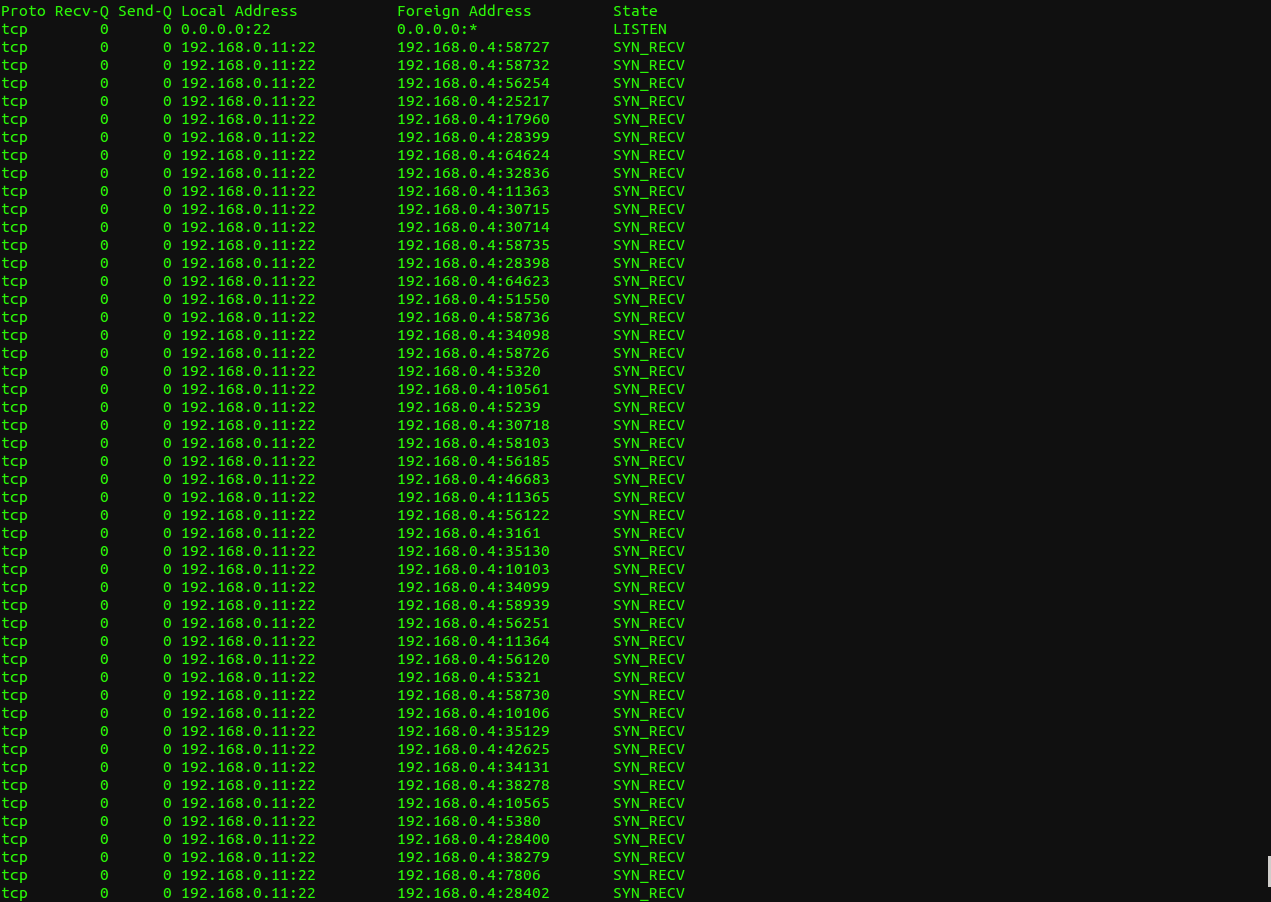
\includegraphics[width=14cm]{tcpsynCookie.png}
\end{center}
\vspace{0.5cm}

\pagebreak
Et si on active la protection : 
\begin{lstlisting}[frame=single,style=Console]  % Start your code-block

echo 1 > /proc/sys/net/ipv4/tcp_syncookies
\end{lstlisting}

Voilà le résultat :
\begin{center} 
\hspace{15cm}
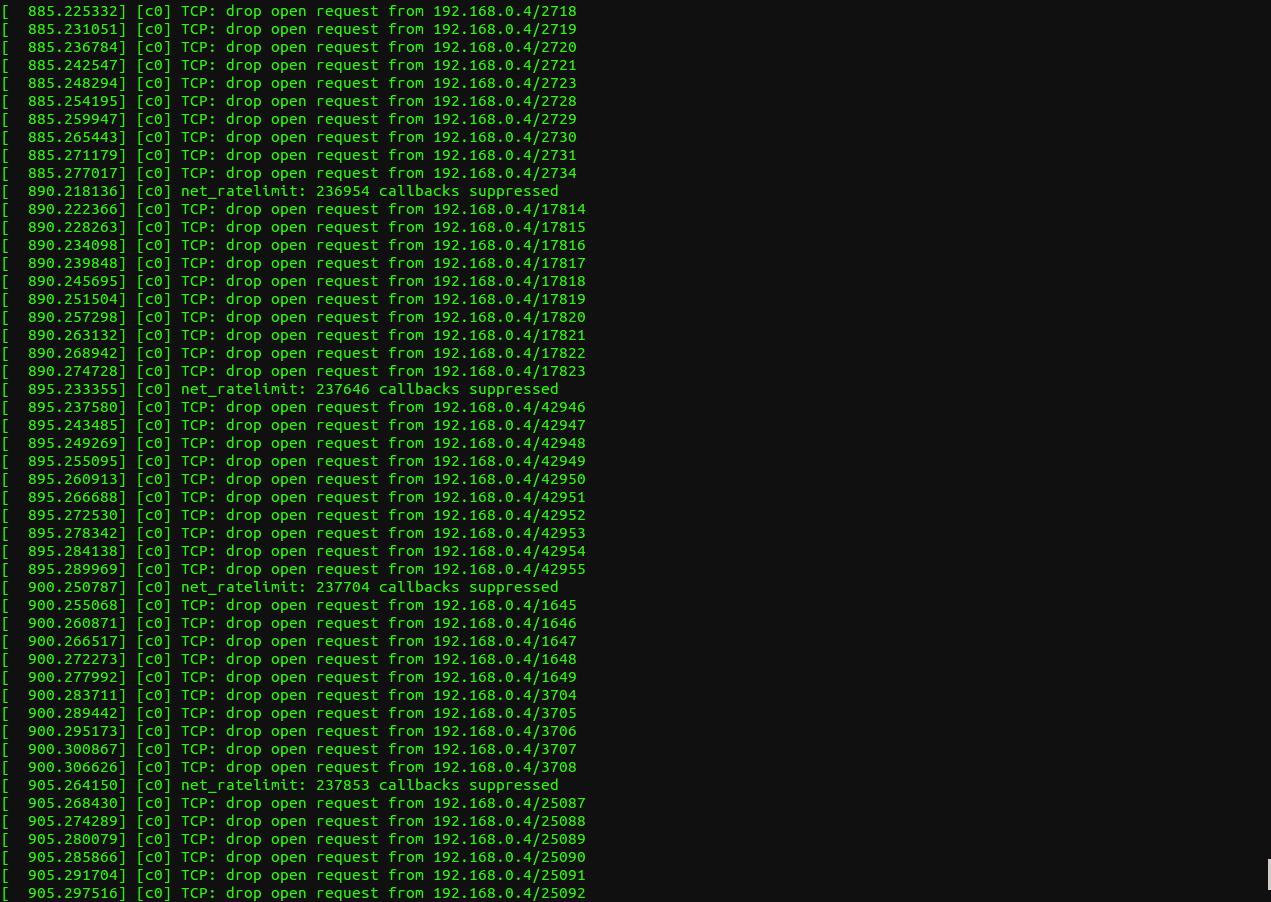
\includegraphics[width=14cm]{tcpSyn_protection.png}
\end{center}
\vspace{0.5cm}

On voit que le noyau rejette les connexions au fur et a mesure qu'elles arrivent et ne se terminent jamais.


